\section{Laser Extrinsic Calibration}
\label{section:laser-extrinsic-calibration}

The key for a good geometric reconstruction is the laser scanner extrinsic calibration, which has to be accurate, so that every point is correctly registered. Therefore, two calibration methods are here presented: the RADLOCC camera-laser calibration (\cref{section:radlocc-method}) and a new method developed in this work (\cref{section:proposed-method}), that aims to achieve better results than the latter. 

\subsection{Radlocc Method}
\label{section:radlocc-method}

\cite{zhang04} presents a method for auto calibration of a camera with a laser scanner. This method, known as Radlocc, uses information from both sensors and tries to find point correspondences to optimize the calibration. In this work, this method was used together with the extrinsic calibration method (explained in section ??), to obtain the full extrinsic laser calibration.

To use this method, the user has to obtain a calibration dataset, which is a set of synchronized images and laser scans containing a chessboard in multiple poses. The chessboard serves as the calibration object, which is the link between the two sensors. In this work, a ROS package was developed to handle this capture and to convert between the ROS messages and the RADLOCC format. Its source code and all documentation can be found in \url{https://github.com/bernardomig/radlocc_calibration}. In the 3D scanner, the laser scanner was positioned such that the laser scans are horizontal and about \numrange{20}{30} images were taken per dataset. Such images are shown in \cref{figure:radlocc-images}.


\begin{figure}
    
    \centering
    \begin{subfigure}{0.5\textwidth}
        \centering
        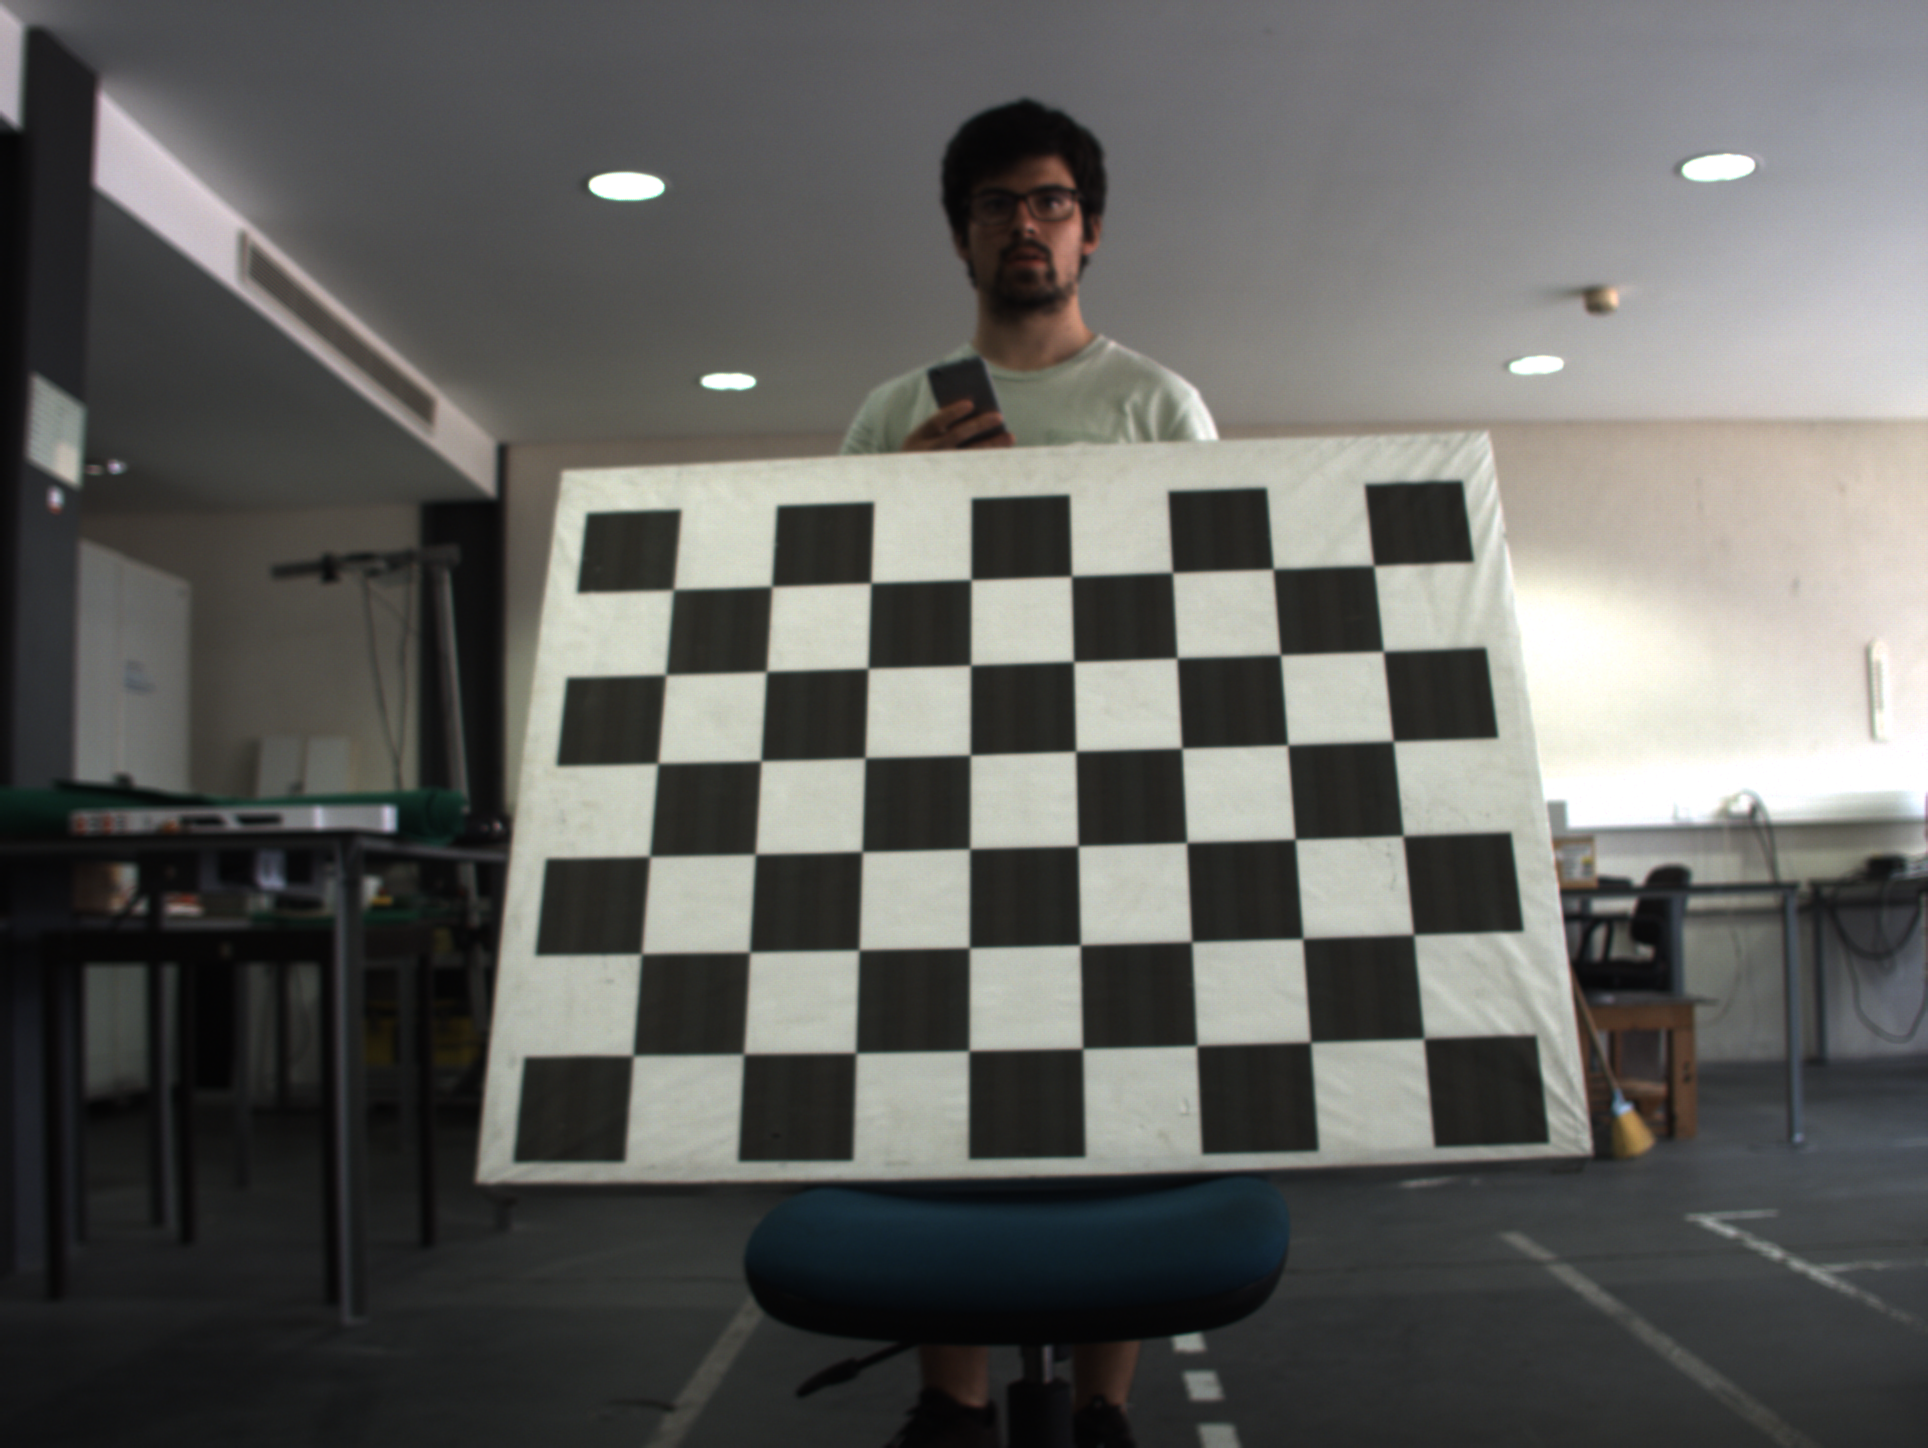
\includegraphics[height=5cm]{radlocc_image_0}
    \end{subfigure}%
    \begin{subfigure}{0.5\textwidth}
        \centering
        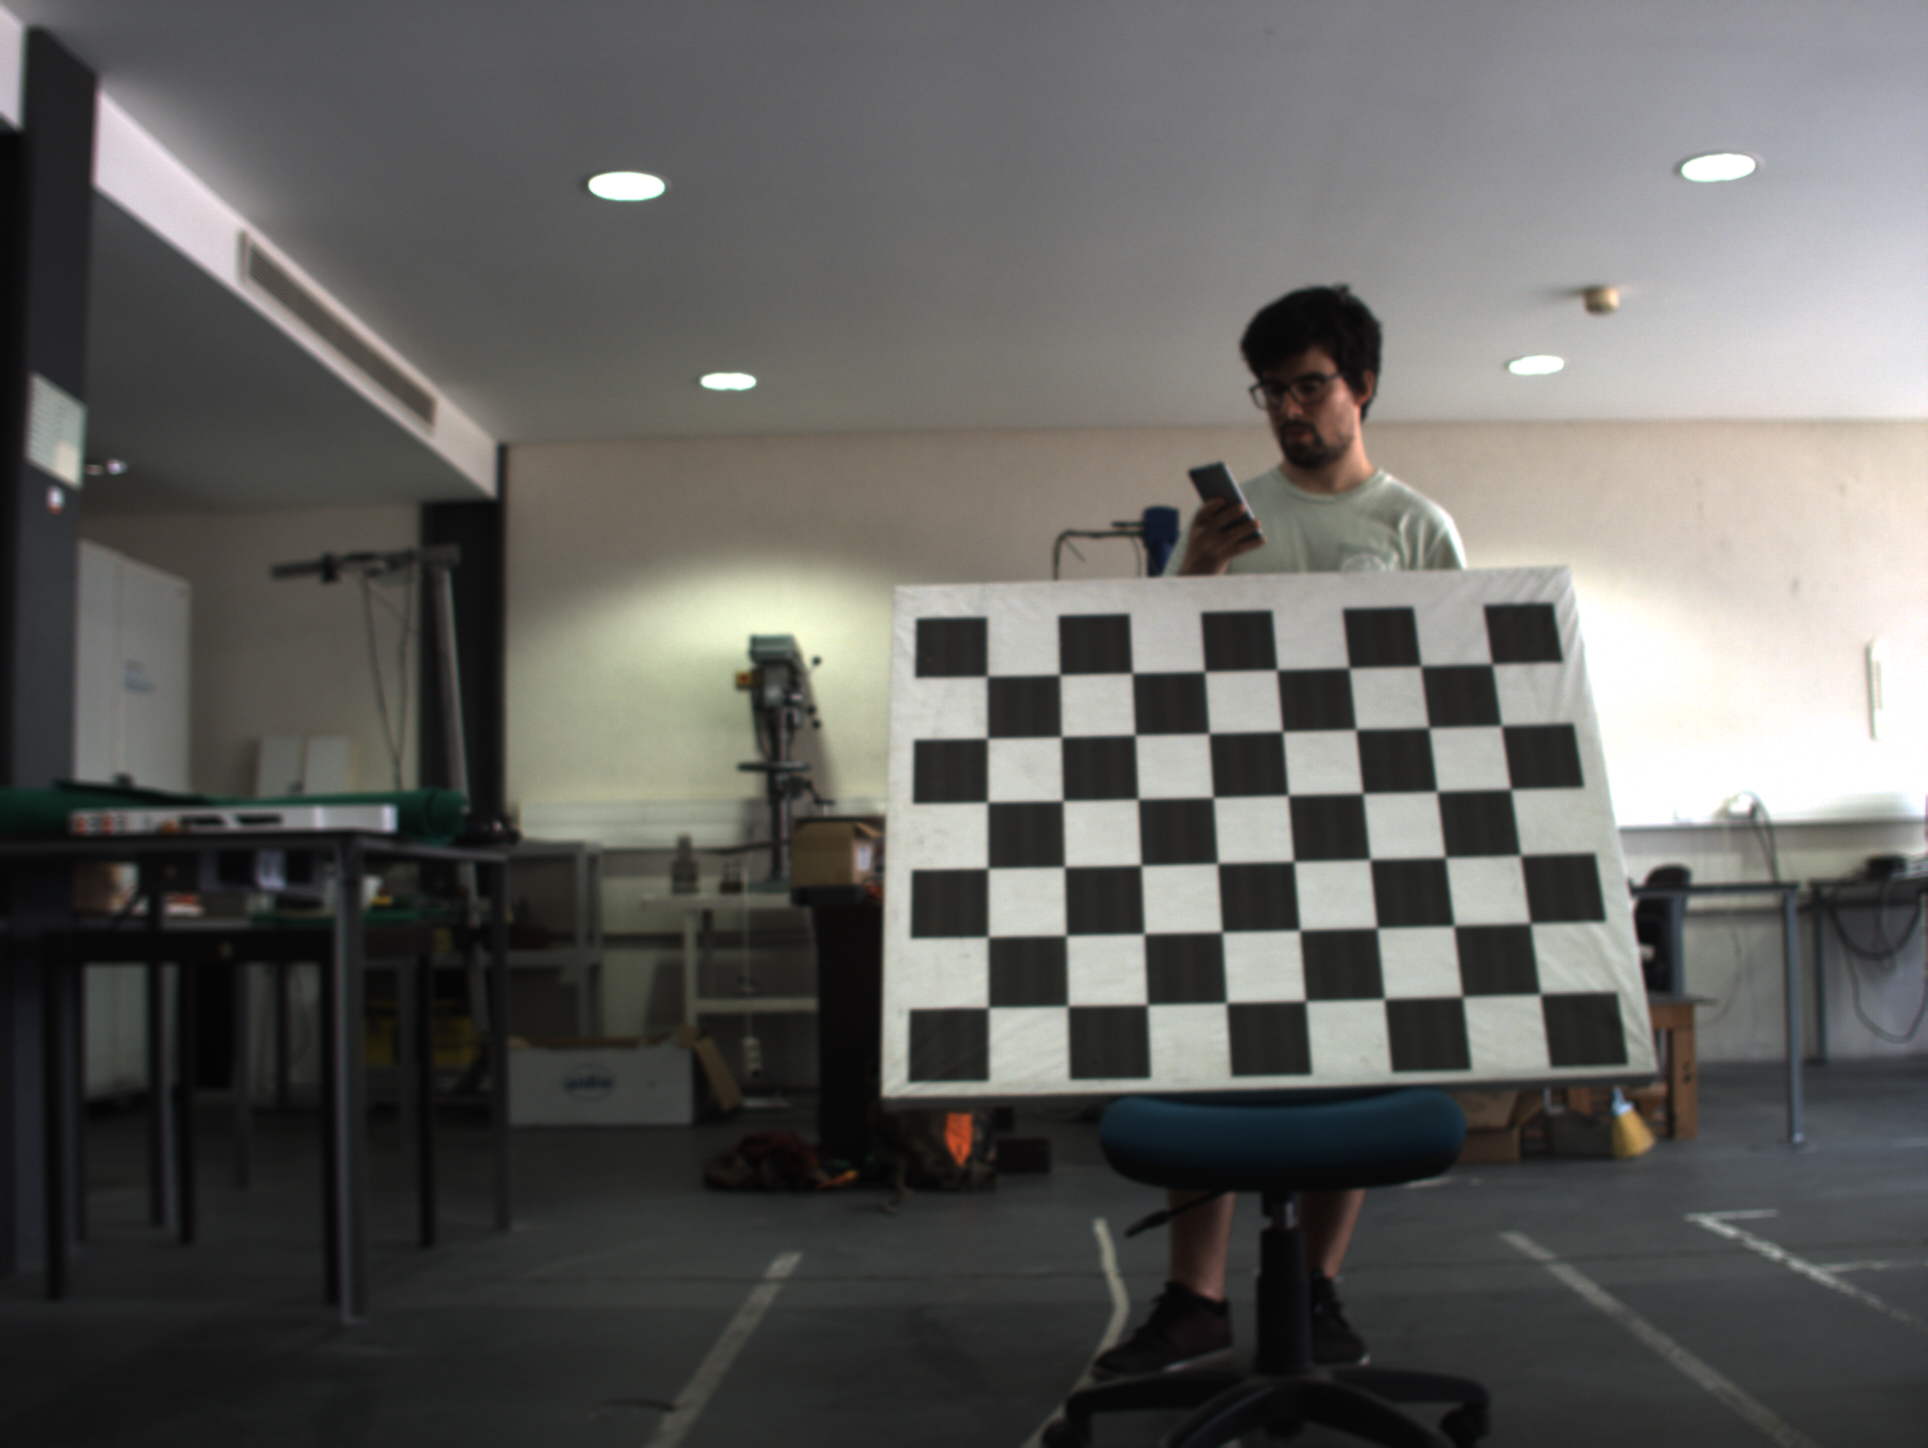
\includegraphics[height=5cm]{radlocc_image_1}
    \end{subfigure}%

    \vspace{1cm}
    
    \begin{subfigure}{0.5\textwidth}
        \centering
        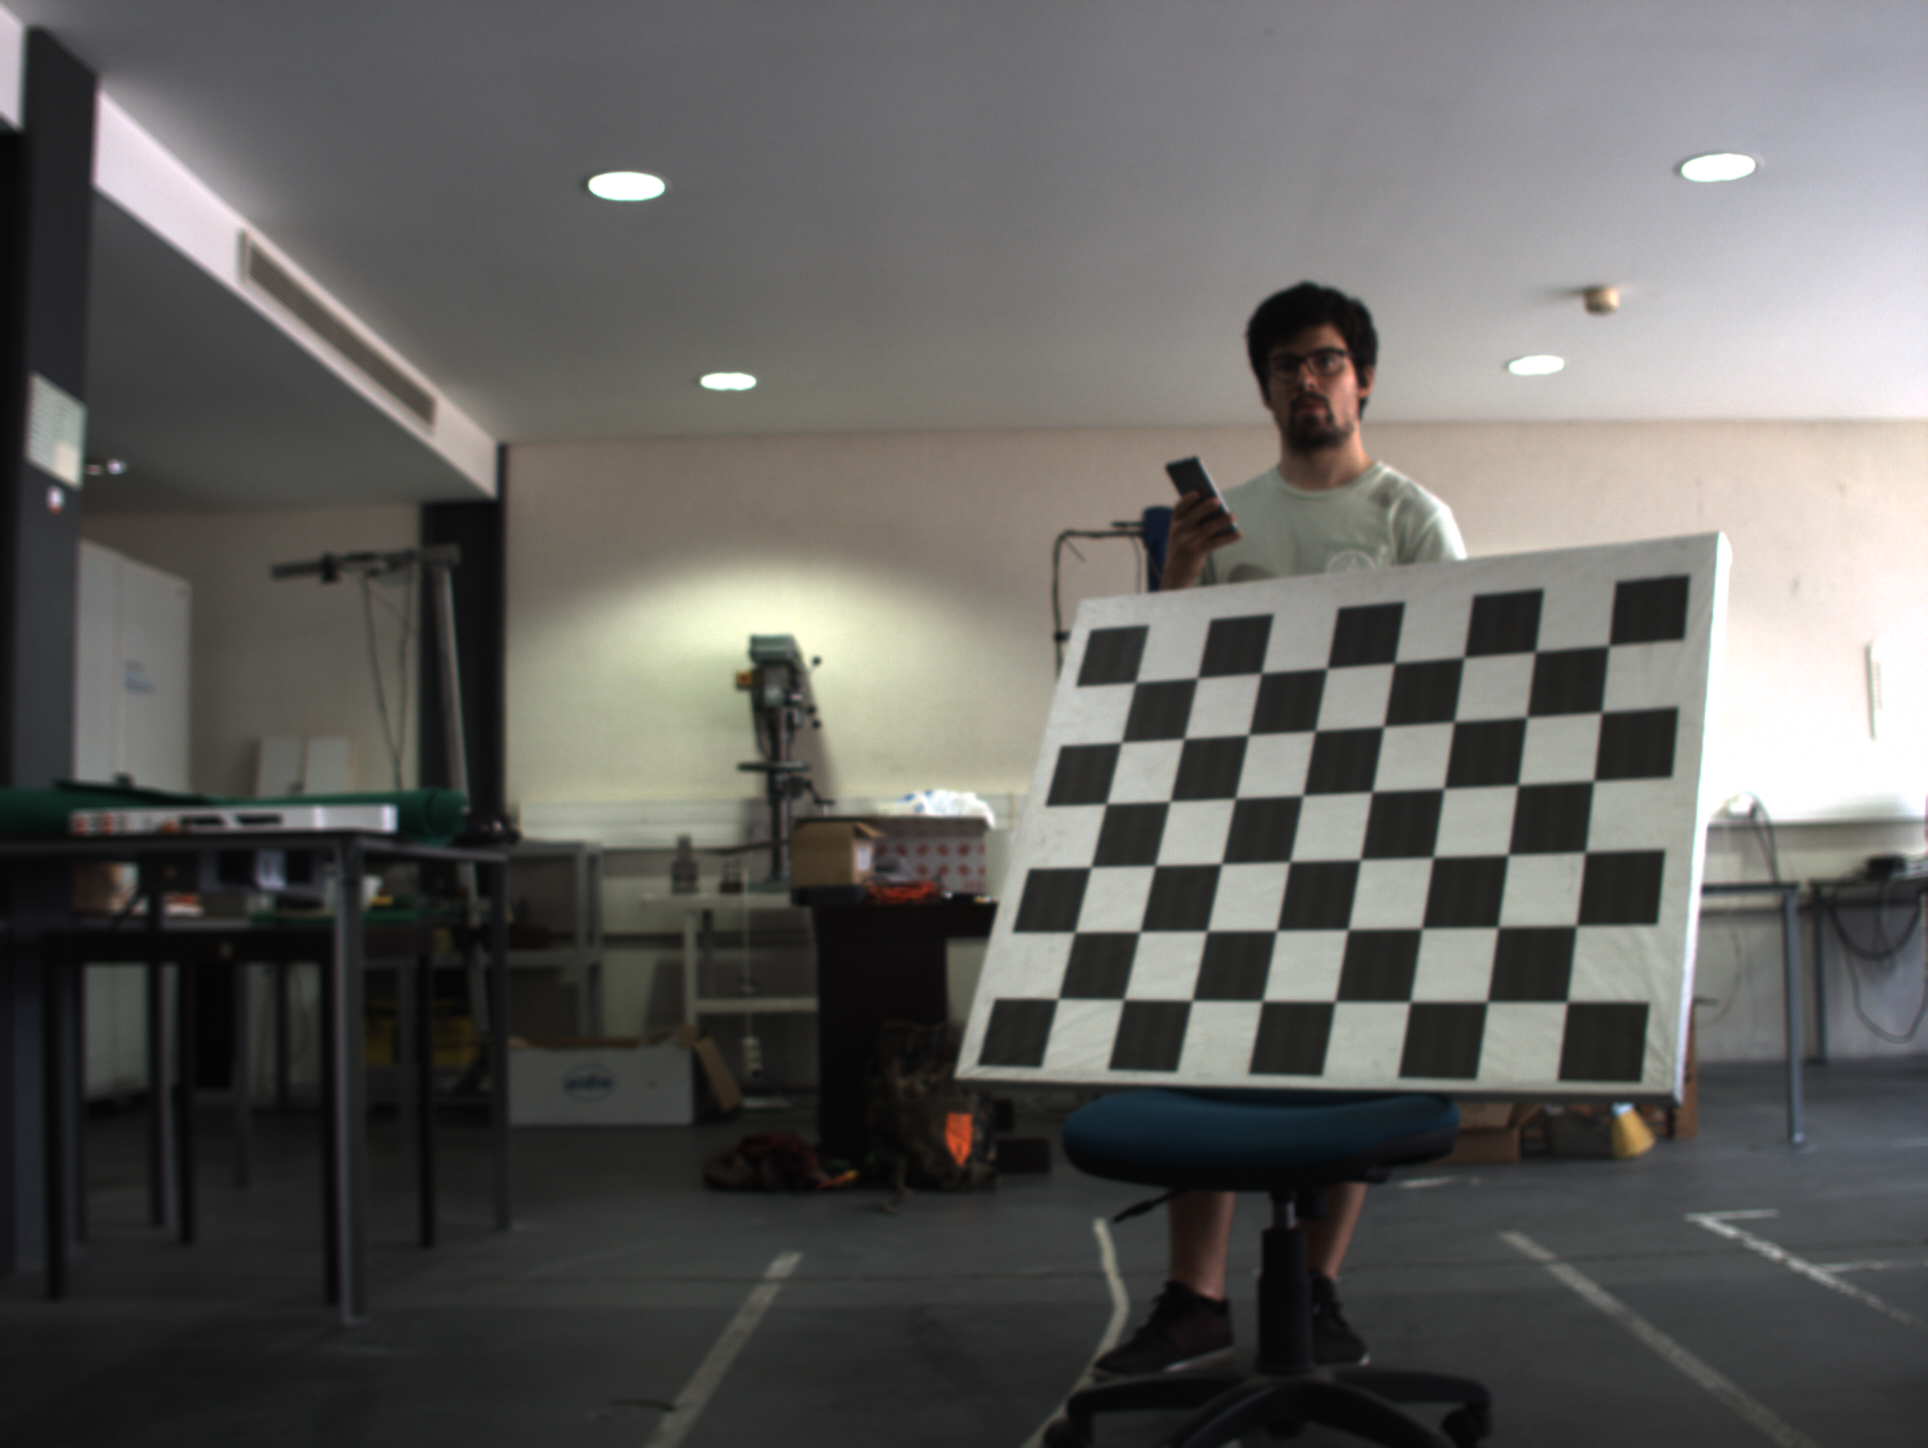
\includegraphics[height=5cm]{radlocc_image_2}
    \end{subfigure}%
    \begin{subfigure}{0.5\textwidth}
        \centering
        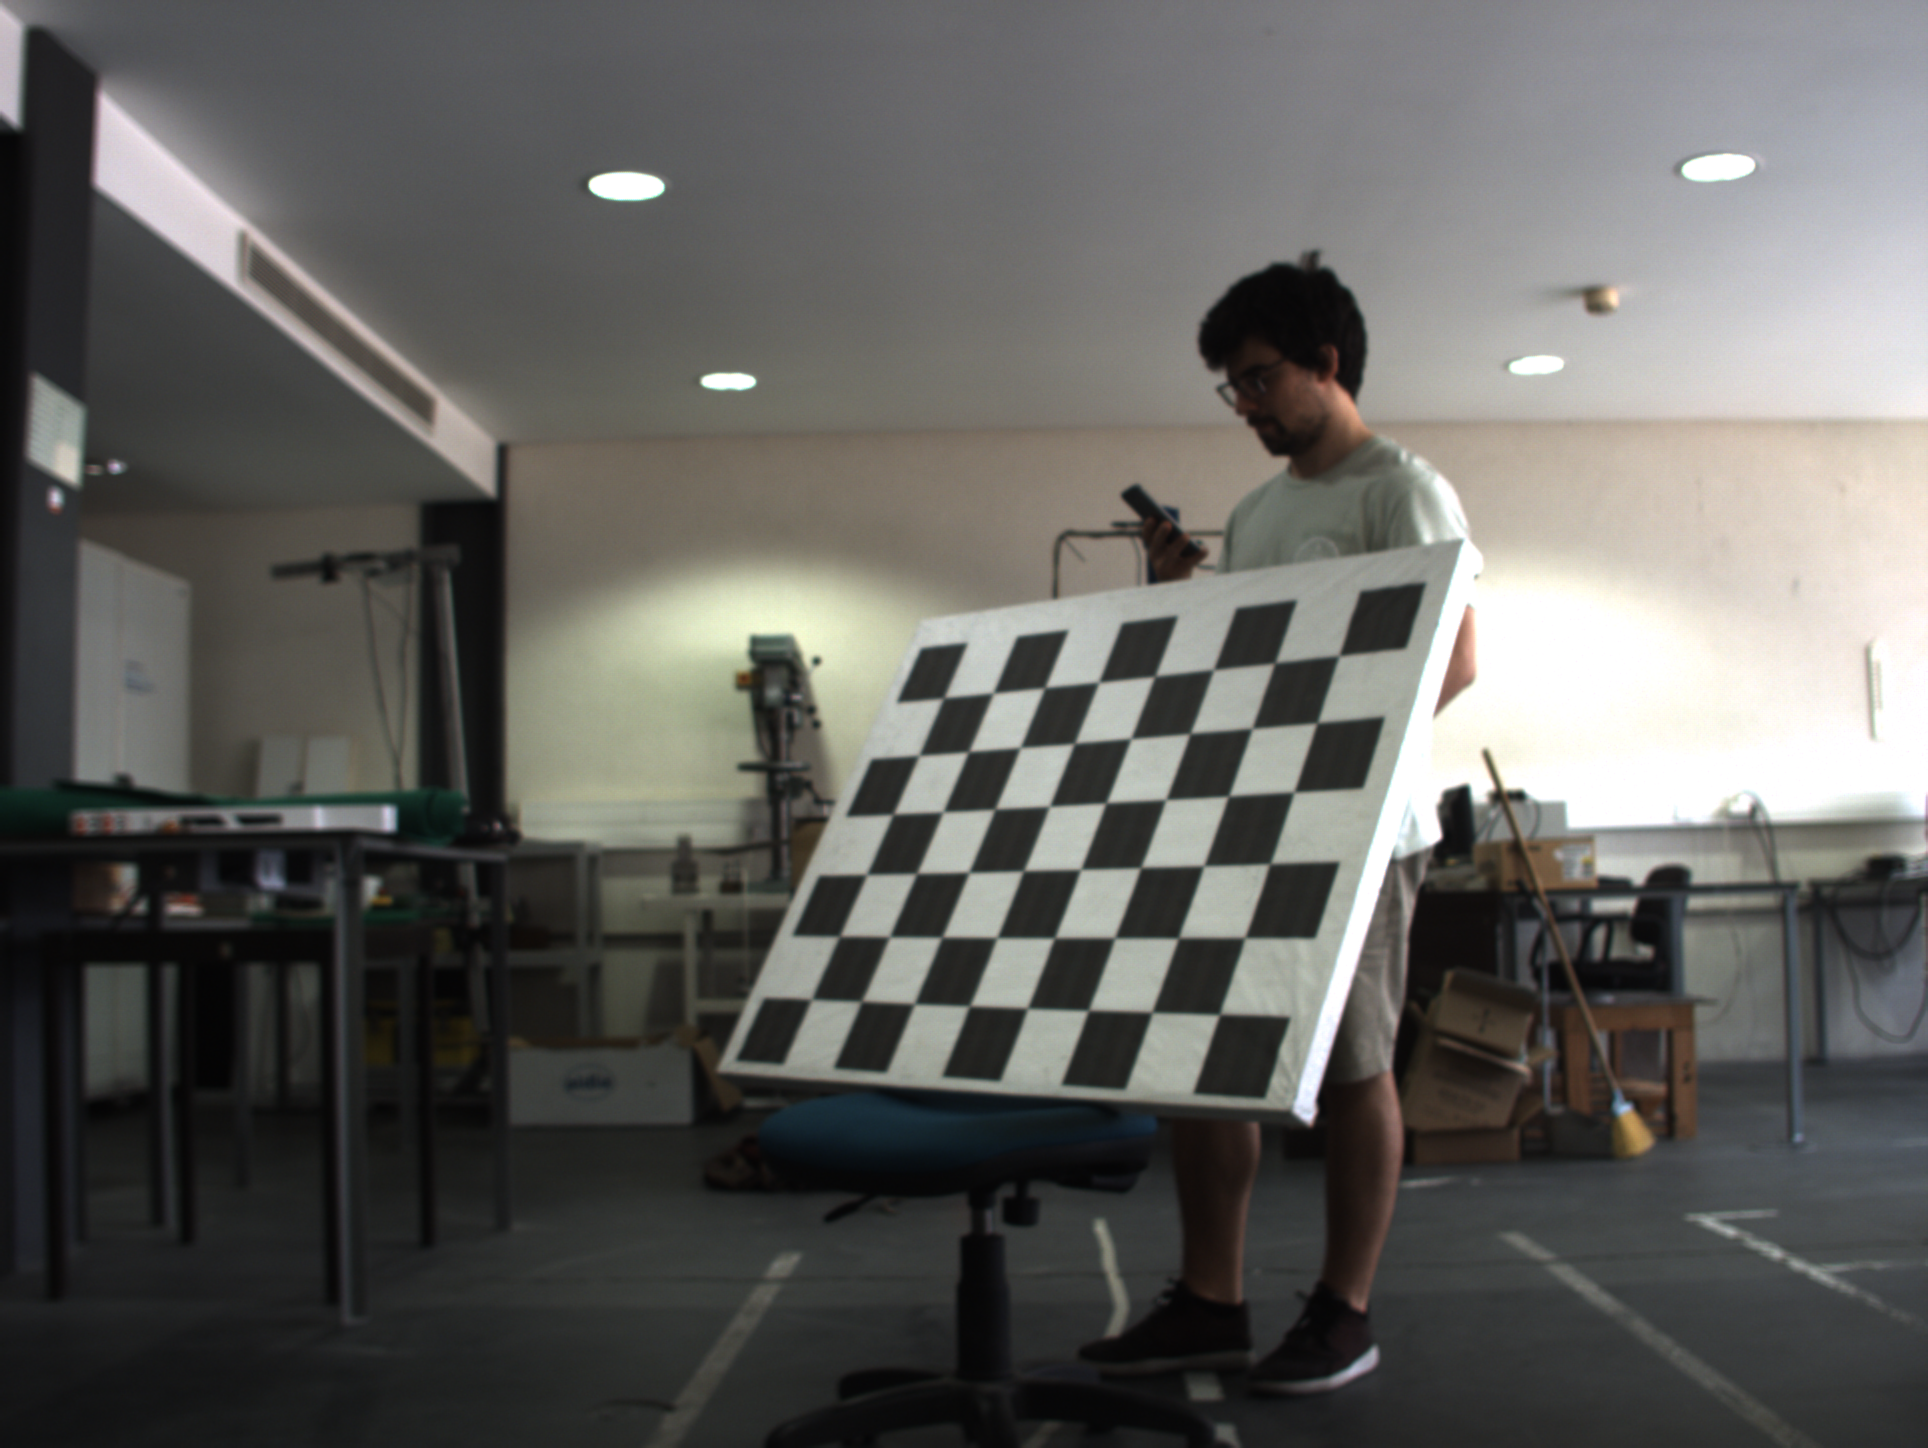
\includegraphics[height=5cm]{radlocc_image_3}
    \end{subfigure}%

    \caption{Images captured for RADLOCC}
    \label{figure:radlocc-images}
\end{figure}

First, a chessboard extraction algorithm finds both finds the intrinsic calibration of the camera, as well as the poses of each chessboard in the camera coordinate frame. Then, laser scans are segmented into board/background, and all the board points are extracted, as seen on \cref{figure:radlocc-points}.

\begin{figure}
    \centering
    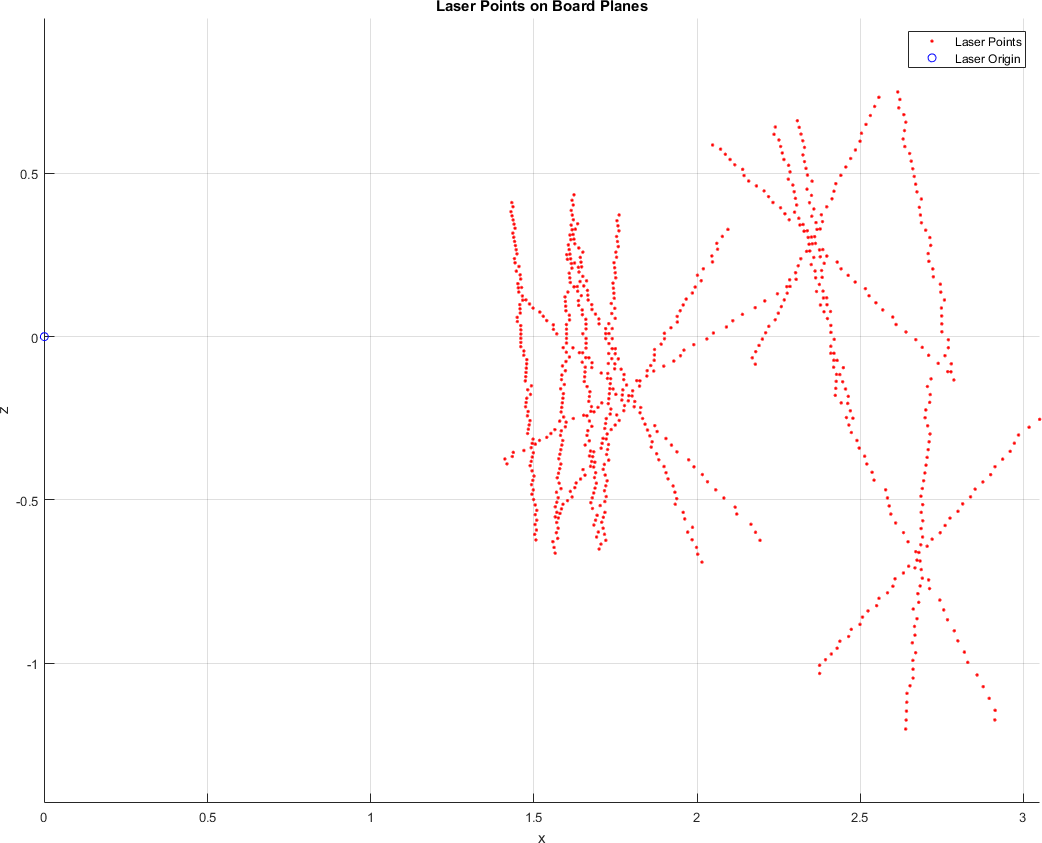
\includegraphics[width=0.5\textwidth]{radlocc_points}
    \caption{Radlocc laser scans chessboard extraction}
    \label{figure:radlocc-points}
\end{figure}

Then, the reprojection error of the laser scans points to the chessboard plane are computed, and the transformation from 

Then, the reprojection error of the laser scans points to the chessboard plane are calculated, depending of the transformation from the camera to the laser scanner. The reprojection error is minimized during the calibration optimization, and the transformation from the camera to the laser if found.

Finally, the extrinsic calibration can be calculated as in \cref{eqn:radlocc-full-calibration}.

\begin{equation}
    \label{eqn:radlocc-full-calibration}
    \mathcal{T}_{calibration} = \TF{PTU}{laser} = \TF{PTU}{camera} \cdot \TF{camera}{laser}
\end{equation}

\subsection{Proposed Method}
\label{section:proposed-method}

A new method was developed in this work to calibrate the laser scanner in this system. One of the key differences to the previous method (in \cref{section:radlocc-method}) is that the calibration is done only using the laser range data, and the calibration from the PTU to the laser scanner is directly find. The hypothesis that this method relies, is that in a good calibration the deviation of a point set is minimal. In other words, in a point set representing a planar surface, the deviation from the points to the planar surface is the lowest, if the extrinsic calibration is the correct one.

This method is, therefore, an optimization problem. For each extrinsic calibration transformation $\mathcal{T}$, corresponds a point cloud $\mathcal{P}$, following the method shown on \cref{section:point-registration}. Then this point cloud is evaluated by a loss function, which determines quantitatively how good each generated point cloud is. Finally, an optimizer will find the transformation $\mathcal{T}$ that minimizes the loss function. Each one of these steps is described in detail next.

\subsubsection{Segmentation}

This calibration method uses an acquisition as its dataset, which is a big advantage. Also, a point cloud has to be generated using a estimation of the calibration transformation. This point cloud does not have to be geometrically accurate but needs to be sufficient for the plane segmentation, which is done manually prior to the calibration. In this work, the software CloudCompare was used to segment the point cloud into multiple planes, and the data was saved as a scalar index in each point. An example of a segmentation can be seen in \cref{figure:cluster-segmentation-1}, where each cluster is represented with a different color.

The segmentation was not done automatically because most segmentation algorithms, for example the RANSAC algorithm, were not capable of achieving a reliable segmentation for the initial estimate, because the point cloud had significant deformation. In addition, manual segmentation is easy to do and accurate, considering that it is a one-time process.

During the optimization, this segmentation serves as a blueprint for all the segmentations. Each point cloud is generated in the same way, so the sequence of points is always the same. Therefore, it is always possible to match any point on the generated point cloud to the point in the segmented point cloud, and get the corresponding cluster index for all the points.

\begin{figure}[h]
    \centering
    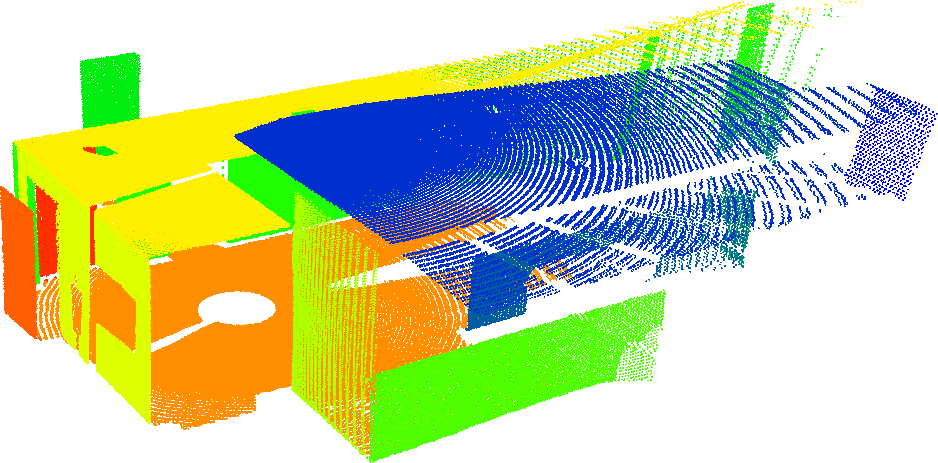
\includegraphics[width=.8\textwidth]{cluster-segmentation-1}
    \caption{Example of a plane segmentation, where each color represents a cluster}
    \label{figure:cluster-segmentation-1}
\end{figure}

\subsubsection{Loss Function}

A loss function, or cost function, is a measure in optimization that compares the result of a model with its expected result, and returns a value that signifies the difference between the two. More concretely, in this calibration the loss function has two components: the loss function per cluster and the loss function per point cloud, which combines the loss of all the clusters. 

To start with, the plane equation for each cluster is found, using the same method as in \cref{section:normal-estimation}, the Principal Component Analysis, or PCA. First the centroid of each plane is found, which is the same as the mean value of all the points $\bar{p}$ (\cref{eqn:centroid-plane}). Then, the covariance matrix $\mathcal{C}$ is calculated (\cref{eqn:covariance-plane}).

\begin{align}
    \bar{p} = & \sum_{i}{p_i}
        \label{eqn:centroid-plane} \\
    \mathcal{C} = & \sum_{i}{(p_i - \bar{p}) \otimes (p_i - \bar{p})}
        \label{eqn:covariance-plane}
\end{align}

Then, the principal axes of the plane is find by an eigen decomposition of the covariance matrix. The smallest eigenvalue $\lambda_3$ will be the variance $\sigma^2$ of the cluster. In other words, $\sigma^2$ is the mean square of the orthogonal distance of all points in the cluster to the plane. So, $\sigma^2$ can be a quantitative factor to measure the loss for each plane. Formally, let us admit that the $\sigma^2$ has two components: the statistical error of the laser sensor $\sigma^2_{sensor}$, which is not affected by the calibration and a second component $\sigma^2_{calib}$, which results from the calibration error. Thus, it is possible that by minimizing $\sigma^2$, a exact calibration can be obtained. For this calibration, however, the value $\sigma$ was used instead of $\sigma^2$, which is known as the Root Mean Square Deviation, or RMS. Therefore, the loss of each cluster will be the $\sigma$ value.

Next, the losses of the clusters are combined into a scalar value, which is the loss of the point cloud. The method found was to, again, calculate the RMS of the values of the partial losses $loss_i$, according to the \cref{eqn:rms}. This value is expected to be minimal when all the partial losses are minimal which, according to this hypothesis, corresponds to a correct calibration.

\begin{equation}
    \label{eqn:rms}
    RMS = \sqrt{\sum_{i}^{N}{x_i^2}}
\end{equation}

\subsubsection{Paramerization}

The parameters in this calibration should define a geometric transformation in space, which is, in the end, a transformation matrix (\cref{eqn:transformation-matrix}). This transformation can be decomposed into two components, a translation and a rotation. The translation can be represented as the vector $t = (t_x, t_y, t_z)$, and the rotation can be represented as a $3 \times 3$ rotation matrix $R$. Since a rotation matrix has only $3 \times 3 = 9$ elements but only 3 degrees of freedom, another parameterization has to be used to represent a rotation. Popular parameterization for rotations are euler angles, quaternions and axis/angle representation. 

\begin{equation}
    \label{eqn:transformation-matrix}
    \mathcal{T} = \left[
        \begin{array}{cccc}
            r_{11} & r_{12} & r_{13} & t_x \\
            r_{21} & r_{22} & r_{23} & t_y \\
            r_{31} & r_{32} & r_{33} & t_z \\
            0      & 0      & 0      & 1   
        \end{array}
    \right]
\end{equation}

However, not all representations are suitable for an optimization. In fact, in~\cite{hornegger99} the term fair parameterization was introduced: a parameterization is called fair, if it does not introduce more numerical sensitivity than the one inherent to the problem itself. Therefore, fair parameterization are a requirement for optimizations, as it increases the changes of convergence. For example, euler angles, which are probably the most used angle parameterization, are not suitable for optimizations~\cite{schmidt01}, because they do not yield smooth movements, each rotation is non-unique and, most notably, there are singularities, so-called \textit{gimbal-lock} singularities, where one degree of freedom is lost~\cite{schmidt01}. Also, quaternions are not suitable for optimizations, because quaternions have $4$ components which are norm-1 constrained. Despite being a fair parameterization, quaternions introduce some complexity in the algorithm to handle the norm-1 constrain, so they are not usually used for optimizations~\cite{schmidt01}.

The axis/angle parameterization is the most widely used to represent a rotation in an optimization, as it is a fair parameterization and has only three components. Any rotation can be represented as a rotation around an axis $a$, by an angle $\theta$. Since $a$ only represent the direction of the rotation (hence only has 2 degrees of freedom), it can be combined with the angle $\theta$ into a single vector $\omega$, as in \cref{eqn:axis-angle}.

\begin{equation}
    \label{eqn:axis-angle}
    \begin{aligned}
        \theta & = |\omega| \\
        a & = \frac{\omega}{|\omega|}
    \end{aligned}
\end{equation}

Computing the rotation matrix from $\omega$ is done using the Rodrigues' formula~(\cref{eqn:rogriguez-1,eqn:rogriguez-2})~\cite{schmidt01}.

\begin{align}
    \label{eqn:rogriguez-1}
    R = I + \frac{\sin \theta}{\theta} [\omega] + \frac{1 - \cos \theta}{\theta^2} [w] \\
    \label{eqn:rogriguez-2}
    [w] = \left[
        \begin{array}{ccc}
            0  & -\omega_3 & \omega_2 \\
            \omega_3 & 0   & -\omega_1 \\
            -\omega_2 & \omega_1 & 0 \\
        \end{array}
    \right]
\end{align}

In conclusion, the parameter vector will have 6 values: 3 representing the translation ($t_1, t_2, t_3$) and 3 representing the rotation in the axis/angle representation ($r_1, r_2, r_3$). So, the parameter vector is shown in \cref{eqn:parameter-vector}.

\begin{equation}
    \label{eqn:parameter-vector}
    P = \{t_1, t_2, t_3, r_1, r_2, r_3\}
\end{equation}

\subsubsection{Optimizer}

The optimization is performed by the Powell's method, described in \cite{powell_method}. This method finds a local minimum of a multi-dimensional unconstrained function, and does not require the gradient of this function, which fits this particular optimization. This method is implemented in the python scientific library SciPy~\cite{scipy-powell}.

\subsubsection{Overview}

To sumarize, the overview of the entire steps of the calibration is shown in \cref{figure:calibration-overview}.

\begin{figure}[h]
    \centering
    \begin{tikzpicture}[
            process/.style={align=center, rotate=90, draw, rectangle, minimum width=4cm},
            data/.style={draw, ellipse},
        ]

        \node[data, anchor=east] (laserscans) at (-2, 0.6) {laserscans};
        \node[data, anchor=east] (transformations) at (-2, -0.6) {transformations};

        \node[data] (parameters) at (0, -4) {parameters};

        \node[process] (registration) at (0,0) {Points \\ Registration};
        \node[process] (segmentation) at (3.5,0) {Segmentation};
        \node[process] (loss) at (7,0) {Loss};

        \node[align=center, draw, rectangle, minimum width=4cm] (optimizer) at (5, -4) {Optimizer};

        \draw[-latex] (laserscans) -- ($(registration.north) + (0,0.6)$);
        \draw[-latex] (transformations) -- ($(registration.north) + (0,-0.6)$);

        \draw[-latex] (parameters) -- (registration);

        \draw[-latex] (registration) -- (segmentation) node[midway, above] {pointcloud};

        \foreach \y in {-1, -0.5, ..., 1} {
            \draw[-latex] ($(segmentation.south) + (0, \y)$) -- ($(loss.north) + (0,\y)$)
                node[midway, above] {cluster};
        };

        \draw[-latex] (loss) -- ++(2, 0) node[midway, above] {loss} |- (optimizer);
        \draw[-latex] (optimizer) -- (parameters);
        
    \end{tikzpicture}

    \caption{Calibration Overview}
    \label{figure:calibration-overview}
\end{figure}
